\documentclass{article}
\usepackage[left=3cm, right=3cm]{geometry}
\usepackage[italian]{babel}
\usepackage{pdfpages, caption}
\usepackage{listings}

\usepackage{hyperref}%for hypertext

\setlength{\footskip}{100pt}

%\usepackage{minted} %for vhdl code

%for clickable table of content
\usepackage{hyperref}
\hypersetup{
	colorlinks,
	citecolor=black,
	filecolor=black,
	linkcolor=black,
	urlcolor=black
}
%opening
\title{Progetto finale di Reti Logiche}
\author{Roland Reylander [10539438]}
\date{1 Aprile 2019}
\begin{document}

\maketitle
\leavevmode
\\[21\baselineskip]
\tableofcontents


\pagebreak

\section{Specifiche di progetto}
Lo scopo del progetto \`e la realizzazione di un componente hardware usando il linguaggio VHDL che risolve il seguente problema: in uno spazio quadrato di 256x256 vengono posizionati 8 centroidi e si vuole trovare il centroide o i centroidi pi\`{u} vicini ad un punto dato.
\newline
Il componente dovr\`{a} interfacciarsi con una memoria RAM dalla quale legge i dati di input e scrive il risultato della computazione. La memoria RAM di input contiene la maschera dei centroidi da considerare, le coordinate dei centroidi, le coordinate del punto dal quale calcolare la distanza e un inidirizzo dedicato al risultato, cio\`{e} la maschera di uscita.
\newline

\renewcommand{\arraystretch}{1.5}
\begin{center}

\begin{tabular}{ |c|c|c| }
	\hline
	INDIRIZZO RAM & CONTENUTO \\ 
	\hline
	0 & maschera dei centroidi \\
	\hline
	1 & coordinata X del centroide \\
	\hline
	2 & coordinata Y del centroide \\
	\hline
	\vdots & \vdots \\
	\hline
	17 & coordinata X del punto da considerare \\
	\hline
	18 & coordinata Y del punto da considerare \\
	\hline
	19 & maschera di output del risultato \\
	\hline
	\vdots & indirizzi non utili \\
	\hline
\end{tabular}
\captionof{table}{Rappresentazione della RAM} 
\end{center}
\leavevmode\newline
Per risolvere il problema \`{e} necessario leggere la maschera e le coordinate del punto e successivamente leggere dalla RAM i centroidi per poi valutare quelli pi\`{u} vicini. Completate queste operazioni bisoga scrivere nell'indirizzo 19 della memoria la maschera che avr\`{a} valore $1$ sul bit relativo al centroide, considerando il bit meno significativo a destra e quello pi\`{u} significativo a sinistra.


\pagebreak
\section{Scelte progettuali}
\label{sec:scelte}
Per affrontare la risoluzione di questo problema \`{e} stata pensata una FSM con i seguenti stati: 
\begin{itemize}
	\item \textbf{reset}: tutti i signal vengono inizializzati;
	\item \textbf{changeAddress}: in base al valore che assume \texttt{cnt} (cio\`{e} \texttt{readMask}, \texttt{readXPoint}, \texttt{readYPoint}, \texttt{readXCoord} e \texttt{readYCoord}) viene aumentato l'indirizzo per la prossima lettura della RAM;
	\item \textbf{waitClock}: la lettura dalla memoria richiede 2 ns e quindi non \`{e} immediata. In questo stato si aspetta un ciclo di clock affinch\'{e} il valore \texttt{i\_data} assuma il valore desiderato che verr\`{a} poi usato nello stato successivo;
	\item \textbf{readData}: in base al valore di \texttt{cnt} in questo stato vengono salvati su dei signal dedicati i valori della maschera e delle coordinate del punto. Successivamente verranno usati i signal \texttt{xAddress} e \texttt{yAddress} per memorizzare le coordinate dei centroidi;
	\item \textbf{calcDistance}: viene calcolata la distanza e memorizzata in \texttt{tempDistance};
	\item \textbf{compareDistance}: la distanza calcolata al punto precedente viene confrontata con \texttt{bestDistance} in modo da tenere solo i centroidi pi\`{u} vicini;
	\item \textbf{sendMask}: \texttt{o\_data} assume il valore del risultato finale, l'indirizzo da mandare alla RAM è il 19$^\circ$ e \texttt{o\_we} viene settato a $1$ per la scrittura del risultato;
	\item \textbf{load}: segnale di \texttt{o\_done} viene messo a $1$ per indicare la fine dell'elaborazione e l'avvenuta scrittura del risultato;
	\item \textbf{last}: \texttt{o\_done} torna a $0$ e il componente torna allo stato di \texttt{reset} pronto per ricevere il prossimo segnale di start.
	
\end{itemize}
Tutto il funzionamento avviene all'interno di un process in cui la lista di sensibilit\`{a} \`{e} composta da \texttt{i\_rst} e \texttt{i\_clk} in modo tale da poter tornare nello stato di \texttt{reset} quando $\texttt{i\_rst}=1$ e osservare il cambiamento del signal \texttt{state} di tipo \texttt{stateType} dichiarato all'inizio.
\newline 
Dopo la lettura della maschera dalla RAM nello stato \texttt{changeAddress} viene scandita la maschera dei centroidi da considerare tramite il signal \texttt{maskPos} in modo da passare alla lettura delle coordinate dei centroidi in caso il bit sia 1 altrimenti verr\`{a} letto il prossimo bit della maschera.
\newline
I signal \texttt{tempDistance} e \texttt{bestDistance} sono entrambi \texttt{std\_logic\_vector(8 DOWNTO 0)} dato che la distanza massima delle coordinate X e Y dei centroidi \`{e} $255+255=510$ e necessita quindi di 8 bit. Inoltre \texttt{bestDistance} viene inizializzata nello stato di \texttt{reset} con \texttt{OTHERS => \textsc{\char13}1\textsc{\char13}} cio\`{e} $511$ che \`{e} maggiore della massima distanza possibile dei centroidi e permettendo il corretto funzionamento dell'algoritmo.
\newline
Nella figura seguente viene rappresentata la macchina a stati mostrando le condizioni significative per passare dallo stato corrente allo stato prossimo. Il cambiamento di stato avviene al ciclo di clock successivo e inoltre da ogni stato è possibile tornare allo stato di reset quando $\texttt{i\_rst}=1$ che non viene rappresentato per non appesantire il grafico.
\pagebreak

\addcontentsline{toc}{subsection}{Macchina a stati}

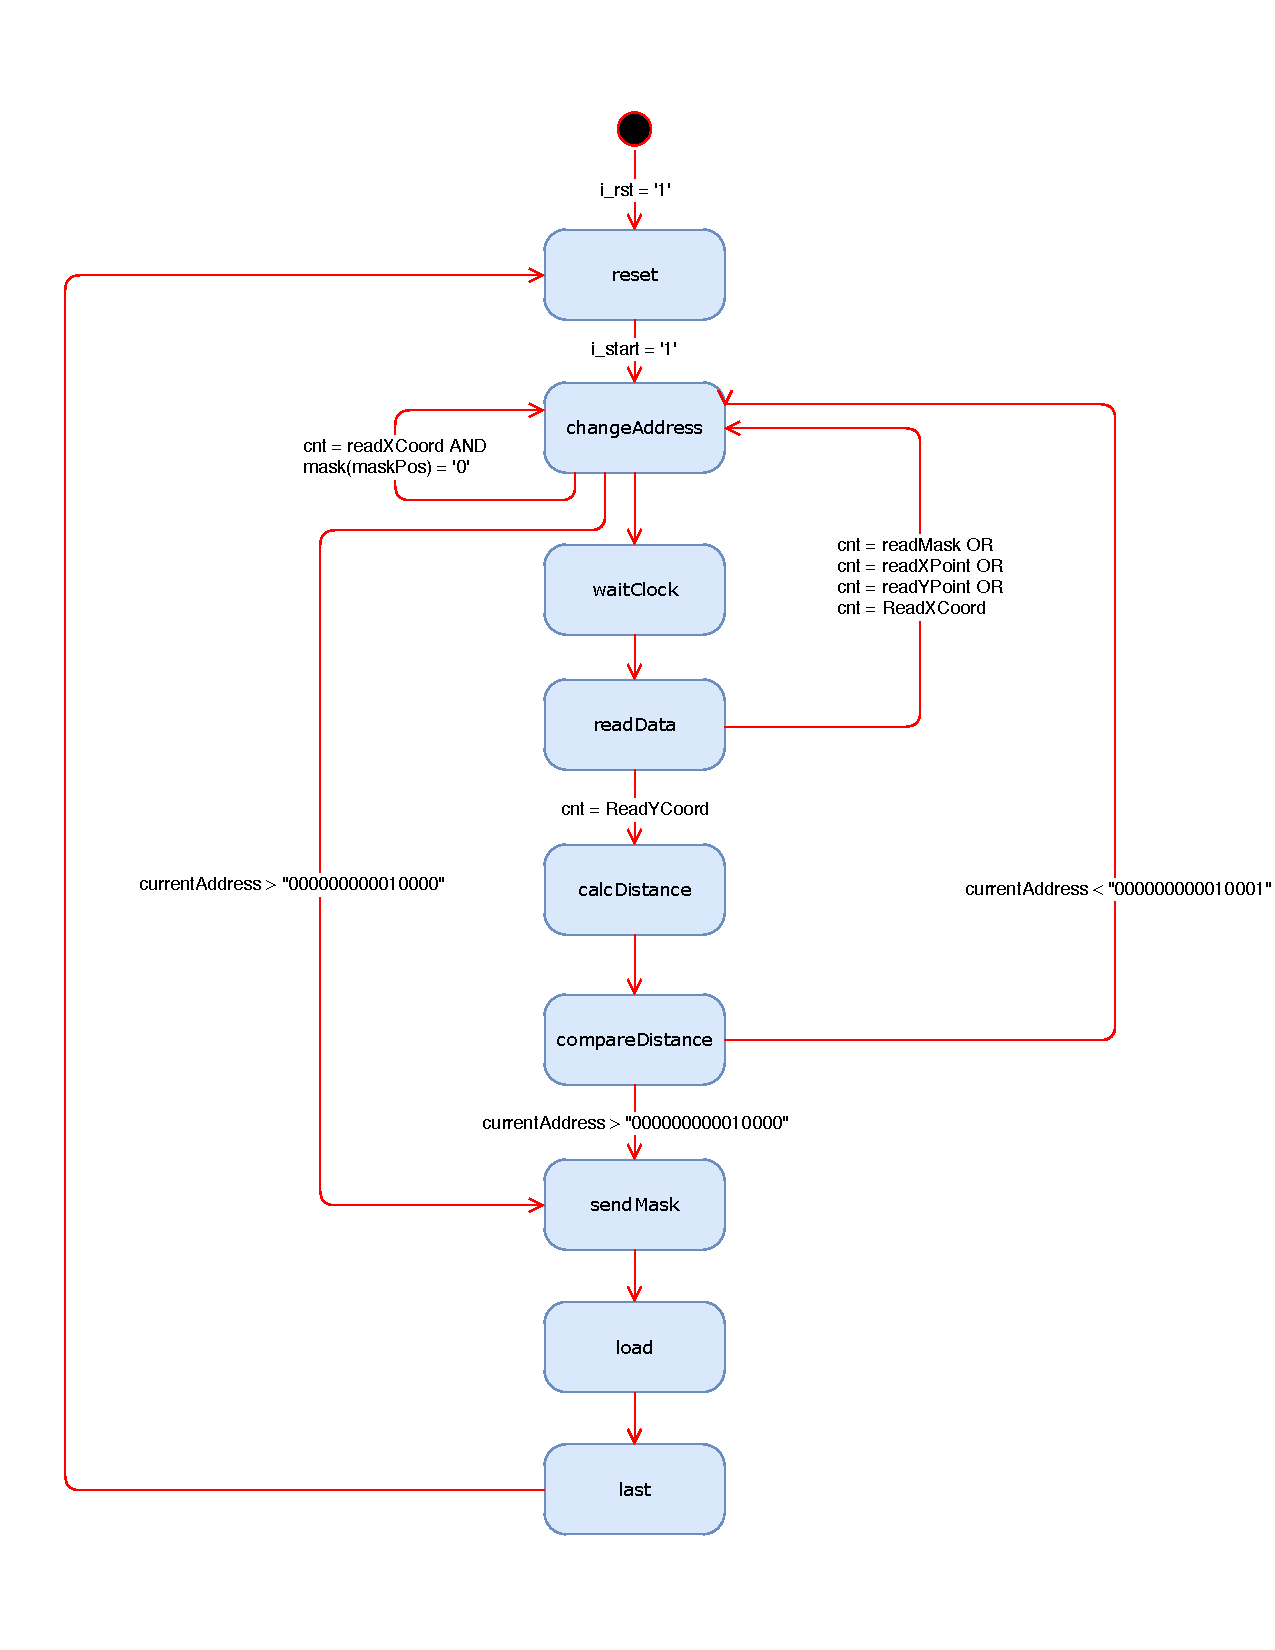
\includepdf[page=-, scale=0.95, offset=0 20, pagecommand={\thispagestyle{plain}\null\enlargethispage{7\baselineskip}\vfill\captionof{figure}{Macchina a stati}}]{diagram.pdf} 
\pagebreak


\section{Risultati dei test}
Per controllare il corretto funzionamento del componente sono stati fatti dei test specifici ogniqualvolta si \`{e} aggiunto un nuovo stato. Questi hanno permesso di controllare che:
\begin{itemize}
	\item gli indirizzi della RAM venissero scanditi uno alla volta partendo da $0$, proseguendo leggendo gli indirizzi $18$ e $19$ per le coordinate del punto. Dopodich\'{e} leggono le coordinate dei centroidi, saltando eventualmente gli indirizzi delle coordinate i cui centroidi hanno il bit della maschera uguale a $0$.
	\item lo stato \texttt{calcDistance} effettivamente calcolasse la distanza giusta, considerando i punti menzionati precedentemente nelle \hyperref[sec:scelte]{\textit{Scelte progettuali}}. Inoltre \`{e} stato controllato che la funzione \texttt{abs()} inclusa nel package \texttt{IEEE.STD\_LOGIC\_1164.all} fosse anche sintetizzable, ottenendo quindi questa formula per il calcolo della distanza:
	\newline
%	\begin{minted}{vhdl}
%	tempDistance <= std_logic_vector((ABS(signed('0' & xAddress) - signed('0' & xPoint)))) +
%	\end{minted}
%	\begin{minted}{vhdl}
%	std_logic_vector((ABS(signed('0' & yAddress) - signed('0' & yPoint))));
%	\end{minted}
	
	
	
	\texttt{tempDistance <= std\_logic\_vector((ABS(signed(\textsc{\char13}0\textsc{\char13} \& xAddress) - signed(\textsc{\char13}0\textsc{\char13} \& xPoint)))) + std\_logic\_vector((ABS(signed(\textsc{\char13}0\textsc{\char13} \& yAddress) - signed(\textsc{\char13}0\textsc{\char13} \& yPoint))));}
	
	\item nello stato \texttt{compareDistance} avvenisse correttamente il confronto tra \texttt{tempDistance} e \texttt{bestDistance} e il passaggio allo stato \texttt{sendMask} dopo il calcolo della distanza dell'ultimo centroide dal punto.
	\item in \texttt{sendMask}, \texttt{load} e \texttt{last} il risultato venisse passato al signal \texttt{o\_data} e successivamente settato \texttt{o\_we}  per la scrittura della RAM.
\end{itemize}
Una volta conclusi i test per verificare la logica del componente si sono aggiunti dei test per il controllo del funzionamento nei casi limite. Il test bench di esepio \`{e} stato quindi modificato con i seguenti cambiamenti:
\begin{itemize}
	\item coordinate casuali e maschere casuali per osservare il funzionamento in generale;
	\item il punto scelto in $(0,0)$ e i centroidi alla massima distanza cio\`{e} $(255,255)$ e il contrario, quindi il punto in $(255,255)$ mentre i centroidi in $(0,0)$. Questo ha permesso di raffinare la formula per il calcolo della distanza.
	\item le coordinate dei centroidi corrispondono con le coordinate del punto dato;
	\item la maschera in ingresso con tutti bit a $0$ e tutti i bit a $1$;
	\item reset casuali per verificare che torni sempre allo stato di \texttt{reset} pronto per iniziare una nuova computazione;	
\end{itemize}


%\begin{minted}{vhdl}
%	process
%	begin
%	CLK <= '1'; wait for 10 NS;
%	CLK <= '0'; wait for 10 NS;
%	end process;
%\end{minted}


\section{Risultati della sintesi}
Il componente passa tutti i test menzionati precedentemente incluso il test bench di esempio. Una volta verificato il perfetto funzionamento in \textit{Behavioral Simulation} il componente \`{e} stato sintetizzato. Dopo la sintesi il componente \`{e} stato sottoposto a tutti i test mostrando risultati sbagliati. Un'analisi attenta ha mostrato che il l'uso di \texttt{variabile} al posto di \texttt{signal} dava dei ritardi inaspettati. La sostituzione delle variabili e una revisione generale del codice hanno portato a una versione finale funzionante. Infatti il componente viene sintetizzato correttamente e passa tutti i test creati sia in \textit{Behavioral Simulation}, in \textit{Post-Synthesis Funcional} e \textit{Post-Synthesis Timing}. Inoltre, anche se non richiesto, il componente passa gli stessi test anche in \textit{Post-Implementation}.

\pagebreak

\addcontentsline{toc}{subsection}{Schema \textit{Post-Synthesis}}

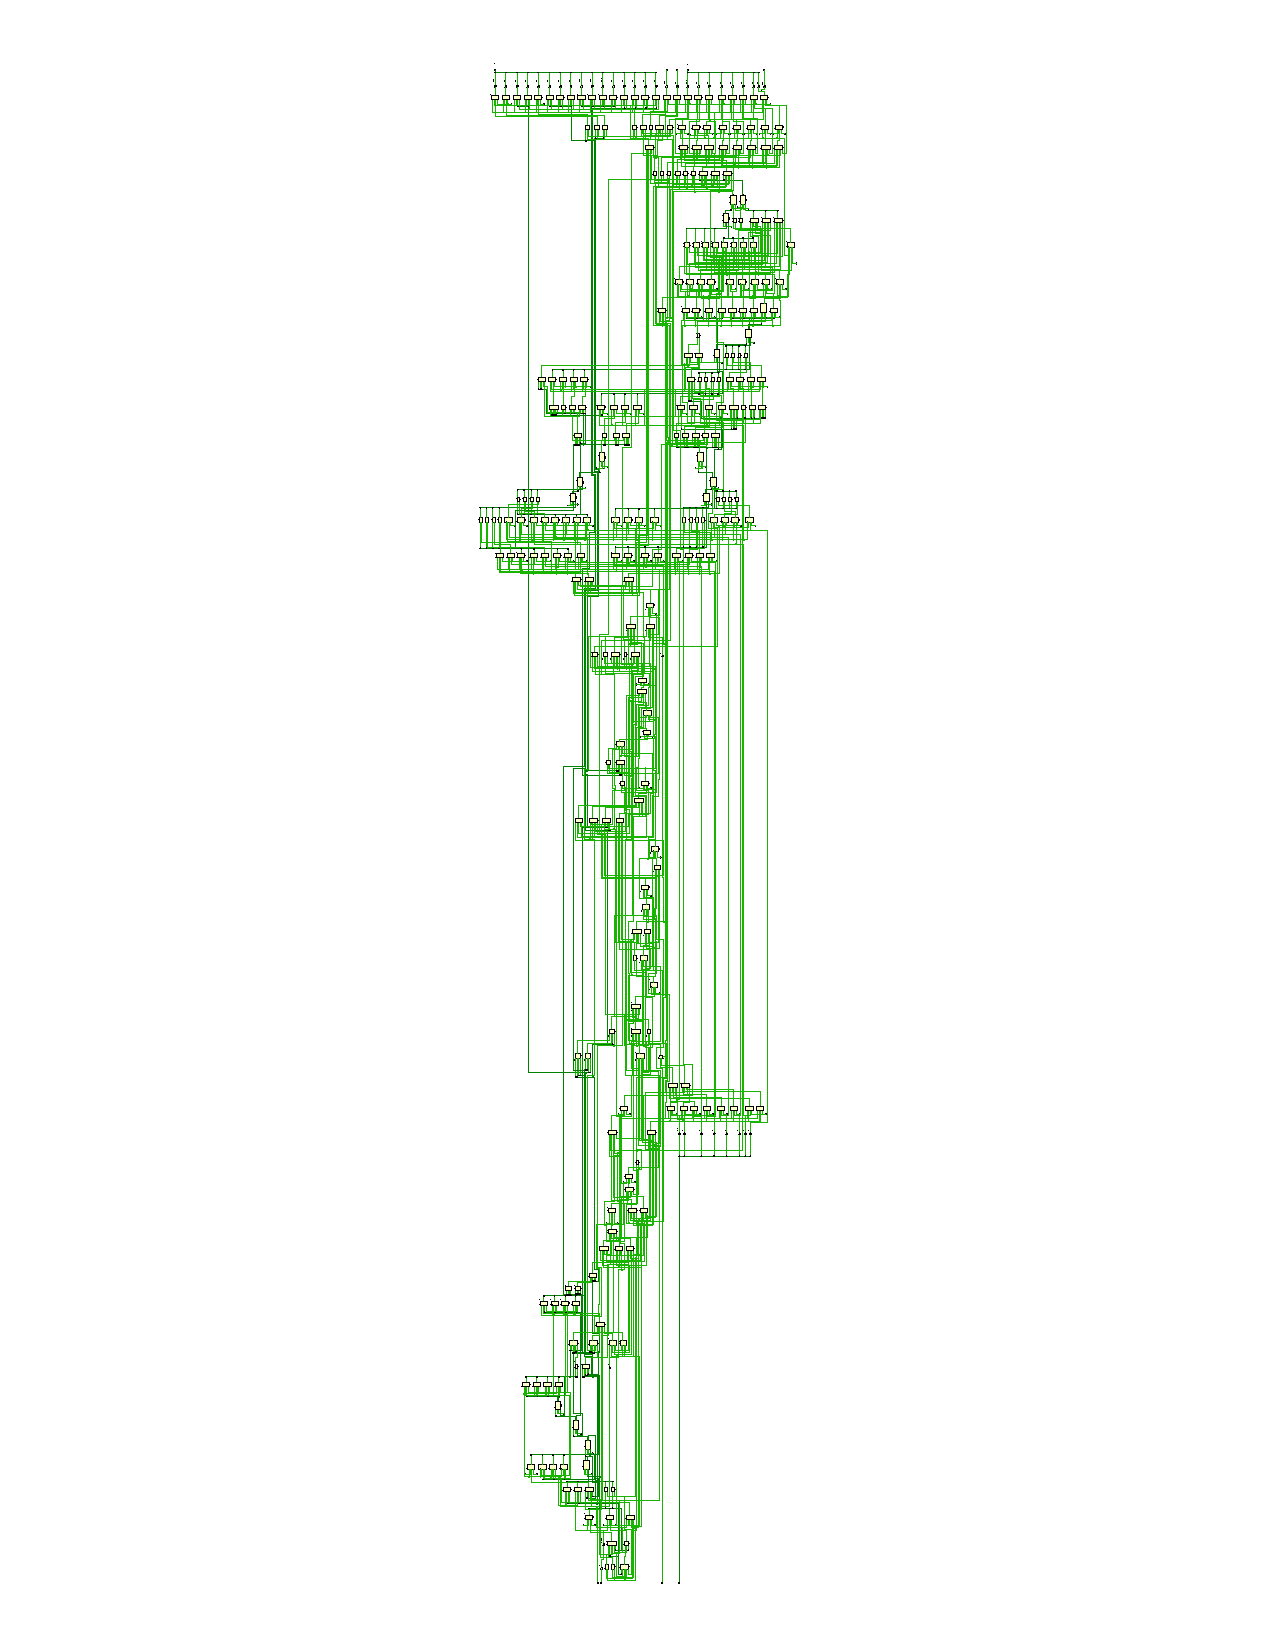
\includepdf[page=-, scale=0.9, offset=0 20, pagecommand={\thispagestyle{plain}\null\enlargethispage{7\baselineskip}\vfill\captionof{figure}{Schema \textit{Post-Synthesis}}}]{schematic.pdf} 
\pagebreak

\end{document}
